\chapterimage{Week5AS.jpg} % Chapter heading image

\chapter{Activated Sludge}

\section{Introduction to Activated Sludge}\index{Introduction to Activated Sludge}
Activated sludge is a secondary, biological treatment process used for the removal of suspended and dissolved organic matter from the primary treated wastewater.
\begin{itemize}
\item Utilizes an aeration basin/reactor and a secondary clarifier

\item In the presence of oxygen, aerobic bacteria in the aeration basin consume the organic matter (BOD) in wastewater for their growth and reproduction, converting BOD into bacterial cell mass along with metabolic byproducts including carbon dioxide and water

\item The aerobic bacteria is the predominant microbial life form in the aeration basin.  Other higher microbial life forms — mainly protozoa, are present along with some metazoans.

\item The microorganisms along with their metabolic byproducts and residual dead cell mass form a cluster called floc.

\item The wastewater exiting the aeration basin enters a clarifier where the floc settles.  The clear, treated secondary effluent flows out.

\item A portion of the settled activated sludge floc, is returned from the clarifier to the front of the aeration basin to seed the activated sludge treatment of the incoming primary effluent. The recycled floc is called \textbf{Return Activated Sludge (RAS)}.

\item The remaining settled floc from the clarifier is ”wasted” \textemdash transferred for solids treatment (typically using digestion) prior to its ultimate disposal. The wasted floc is called \textbf{Waste Activated Sludge (WAS)}.

\item The color of healthy activated sludge is tan to brown with an earthy/musty odor.
\newpage
\begin{center}
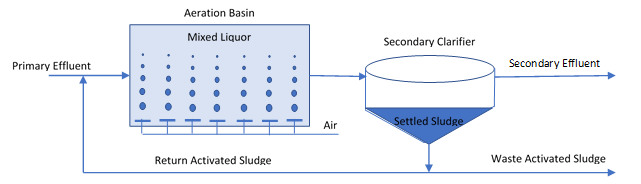
\includegraphics[scale=0.8]{ASProcess}
\end{center}

\item For activated sludge treatment to be effective, it is critical to establish a healthy microbial population which \hl{converts the BOD} into \hl{easily separable biomass.}
\item If the biomass does not settle well in the clarifier, it will be carried out in the treated secondary effluent producing a poor quality effluent with higher solids and organic content.  \\

\item Mixed liquor:
\begin{itemize}
\item Mixed liquor is the mixture of raw and/or treated wastewater with the biomass.
\item Mixed liquor sample is typically taken at the end of the aeration reactor.
\item In the mixed liquor, the suspended solids comprised mostly of biomass with some undegraded and non-degradable material is called \textbf{Mixed liquor suspended solids (MLSS)}.  
\item The volatile fraction of the MLSS is termed \textbf{Mixed Liquor Volatile Solids (MLVSS)}.  \item The MLVSS is the amount of biomass as a percentage of the MLSS.  Generally, the MLVSS is 70 - 80\%, implying that 70-80\% of the MLSS is volatile (organic) solids.
\end{itemize}

\end{itemize}

		\section{Process parameters}\index{Process parameters}
\subsection{Dissolved oxygen (DO)}\index{Dissolved oxygen}%$$$$$$$$$$$$$$$$$$$$%
Maintaining adequate \textbf{Dissolved oxygen (DO)} is key to the activated sludge process.  DO is typically maintained between 0.5 to 3.0 mg/l in the aeration reactor.\\
\subsection{pH}\index{pH}%$$$$$$$$$$$$$$$$$$$$%
The microbiological population in the activated sludge is very sensitive to pH and needs to be maintained at neutral - 7 pH.
\subsection{Temperature}\index{Temperature}%$$$$$$$$$$$$$$$$$$$$%
Biological activity is temperature dependent.  Microbial activity approximately doubles for every 10$^o$C rise in temperature.\\
\subsection{Oxygen uptake rate (OUR) and specific oxygen uptake rate (SOUR)}\index{Oxygen uptake rate (OUR) and specific oxygen uptake rate (SOUR)}%$$$$$$$$$$$$$$$$$$$$%

Oxygen Uptake Rate (OUR) involves measurement of the amount of oxygen used up by the microorganisms using a DO probe and is expressed in unit time of mg/L-hr (ppm O$_2$ consumed per hour). By knowing the OUR, we can establish the activity of the microorganisms in the aeration tank and know if they are consuming the oxygen provided for removing organic matter.  \hl{For conventional activated sludge process the typical OUR values range from 10 to 30 mg/L-hr}\\

Specific Oxygen Uptake Rate (SOUR) provides the OUR information based on the concentration of microorganisms present. SOUR is obtained by dividing OUR with MLVSS. The value is indicated and measured in terms of unit of $\dfrac{\dfrac{mg}{l-hr}O_2}{\dfrac{mg}{l}MLVSS}*1000\dfrac{mg}{gm}$.\\ \hl{Optimal range of SOUR is usually between 8 to 20.}\\
If a baseline OUR is established for a system - presence of toxic susbstances in that system can be identified by a drop in OUR. SOUR value above the optimal range indicates an increasing F:M - Higher BOD load with less than adequate microorganisms (represented by MLVSS) indicating a young sludge and the potential for straggler floc.  A lower than optimal SOUR value indicates insufficient food to support the microorganisms indicating an older sludge and the potential for pin floc.

\subsection{Food to Mass ratio (F:M)}\index{Food to Mass Ratio (F:M)}
In order to establish the amount of the MLSS to be maintained in the aeration tank, the parameter \textbf{Food to Mass Ratio (F:M)} is used.  F:M is the ratio of the "food" – the mass of primary effluent BOD entering the aeration basin to the mass of the microorganisms in the aeration basin \textemdash MLVSS.  Common ranges for F:M for a conventional activated sludge plant are from 0.15 to 0.5\\
\subsection{Sludge age}\index{Sludge Age}

\begin{itemize}
\item Sludge age is the average time (days) that a sludge particle (cell) spends in the system.  \item Sludge age dictates the presence and predominance of the different types of organisms and is measured as Mean Cell Retention Time (MCRT) or Solids Retention Time (SRT).\\
\item Sludge age is the average time that a sludge particle (cell) spends in the system
\item Conventional AS process - MCRTs are in the range of 5 to 15 days
\item The desired MCRT for a given plant must be found experimentally
\item \hl{F:M and MCRT are inversely related: that is a long MCRT means a low F:M and a short MCRT means a high F:M} 
\item Both, F:M and MCRT values vary from plant to plant and are established through a trial and error process.
\item The MCRT is calculated as:\\ 
\end{itemize}

\vspace{0.2cm}
$MCRT(days) = $\\
$\frac{Total \enspace MLSS \enspace lbs \enspace in \enspace the \enspace aeration \enspace system \enspace (aeration \enspace tank \enspace + \enspace clarifier)}{Total \enspace amount \enspace in \enspace lbs/day \enspace of \enspace suspended \enspace solids \enspace leaving  \enspace the \enspace system \enspace(Effluent\enspace SS+ WAS \enspace solids)}$\\
\vspace{0.4cm} 
$MCRT (days) = \frac{MLSS \enspace in \enspace aeration \enspace tank \enspace (lbs)+MLSS \enspace in \enspace clarifier \enspace (lbs)}{Effluent \enspace suspended \enspace solids \enspace (lbs/day)+\enspace WAS \enspace SS \enspace (lbs/day)}$

\subsection{Sludge settleability}\index{Sludge settleability}
\vspace{5mm}
\begin{itemize}
\item A settleability test is conducted on the mixed liquor from the aeration reactor to  measure the compaction and settleability characteristics of the secondary solids.
\item In the settleability test, a 1-liter mixed liquor sample is allowed to settle for 30-minutes in a graduated cylinder $-$ settleometer. 
\item The \textbf{Sludge Volume Index (SVI)} of the sludge is calculated using results from the 30-minute settleability test and the MLSS value.
\item SVI is expressed in ml/g and it is essentially the volume (ml) of 1 gram of the MLSS after 30 minutes of settling.
\item SVI (ml/g)= $\frac{Settled \enspace sludge \enspace volume \enspace in \enspace ml/l \enspace after \enspace 30 \enspace min}{MLSS \enspace mg/l}*1000 \frac{mg}{g}$
\item SVI provides a more accurate picture of the sludge settling characteristics than settleability or MLSS alone.
\item 50 to 120 ml/g SVI value is considered optimal.
\item Higher SVI values  indicate sludge that is slow to settle and not compacting well.
\item When SVI values are approaching 200 ml/g, activated sludge process is considered to be "bulking".
\item Regular monitoring of SVI help identify changes occurring in the activated sludge process preventing settling problems before they occur.
\item Like F:M and MCRT, the optimal SVI value for each plant varies and is also established by trial and error.

\subsection{RAS and WAS Pumping Rates}\index{RAS and WAS Pumping Rates}
The RAS and WAS pumping rates are primarily to control the amount of microbes in the aeration basin and the sludge age.  RAS and WAS adjustments may be necessary to prevent solids build-up in the clarifier which may lead to solids overflowing  with the effluent. Typical RAS flow rates range from 30-100\% of the influent flow rate.
\end{itemize}

		\section{Microbiology}\index{Microbiology}
		
Bacteria are fundamental microorganisms in the stabilization of organic wastes and therefore of basic importance in the secondary wastewater treatment process.  

Bacteria (singular, bacterium) are single celled organisms and represent the simplest forms of life.  These organisms utilize soluble food and are capable of self-reproduction.  
Bacteria can be classified in many different ways. 

For wastewater bacteria are classified based on nutritive requirement, bacteria are classified as heterotrophic or autotrophic bacteria, although several species may function both.

\begin{enumerate}[1.]
\item \textbf{Heterotrophic bacteria} use carbon based organic compounds for both energy and food source. A term commonly used instead of heterotroph is “saprophyte” which refers to an organism that lives on dead or decaying organic matter. The heterotrophic bacteria are grouped into three classifications, depending upon their action toward free oxygen.

\begin{enumerate}[a.]
\item
Aerobes : Require free dissolved oxygen to live and multiply. 
\item
Anaerobes : Oxidize organic matter in the complete absence of dissolved oxygen.
\item
Facultative : Use free dissolved oxygen when available but can also respire and multiply in its absence, e.g. Escheichia coli.
\end{enumerate}

\item \textbf{Autotrophic bacteria} use carbon dioxide as a carbon source and oxidize inorganic compounds for energy. Autotrophs of greatest significance in wastewater treatment are the nitrifying and sulfur bacteria.

\begin{enumerate}[a.]
\item Nitrifying bacteria : These bacteria are responsible for the oxidation of ammonia in wastewater to nitrates. 
\item Sulfur bacteria : These bacteria are involved in the formation of sulfuric acid from the dissolved sulfides in the sewer conveyance systems.
\end{enumerate}
\end{enumerate}

The activated sludge is a complex ecosystem of aerobic microorganisms predominantly heterotrophic bacteria along with some autotrophic bacteria and other \hl{trophic organisms} including \hl{protozoas, rotifers and nematodes} which feed on the bacteria and particulate matter.

Protozoa are single-celled microscopic organisms, several hundred times larger than bacteria. \hl{It is the protozoa we observe under a microscope since bacteria are actually too small to see.} There are four types of protozoa commonly found in activated sludge systems. They are identified by their method of movement within the wastewater environment. The four types are:
\newpage
\begin{tabular}{  m {7 cm}  m {7 cm} } 
\begin{center} 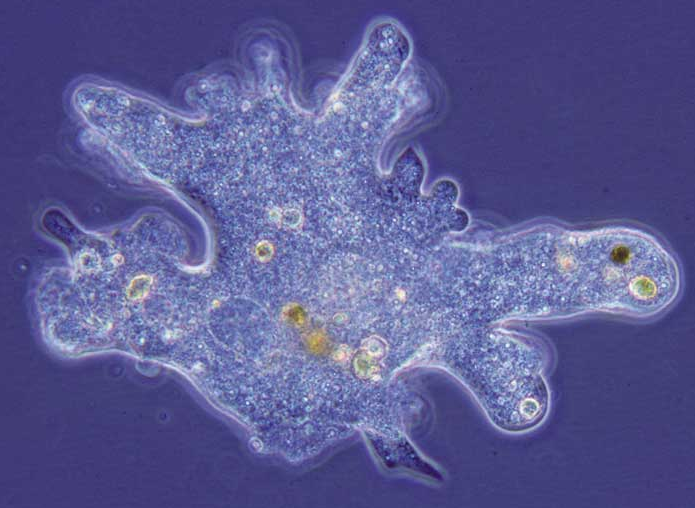
\includegraphics[scale=0.35]{Amoeba} \end{center} & \begin{center}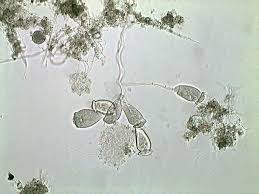
\includegraphics[scale=0.88]{StalkedCilliate} \end{center}\\
\begin{center} \textbf{Amoeba} \end{center} & \begin{center}\textbf{StalkedCilliate} \end{center}\\
\begin{center} 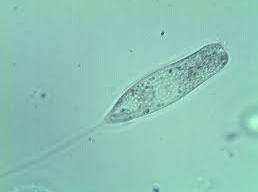
\includegraphics[scale=0.88]{Flagellate} \end{center} & \begin{center}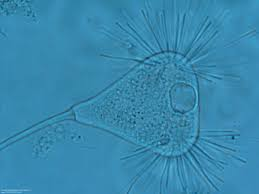
\includegraphics[scale=0.88]{Suctorian} \end{center}\\
\begin{center} \textbf{Flagellate} \end{center} & \begin{center}\textbf{Suctorian} \end{center}\\
\end{tabular}
Other commonly found organisms included the multi-celled organisms - Metazoans such as Rotifers and Nematodes\\
\begin{tabular}{  m {7 cm}  m {7 cm} } 
\begin{center} 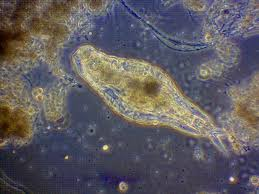
\includegraphics[scale=0.875]{Rotifer} \end{center} & \begin{center}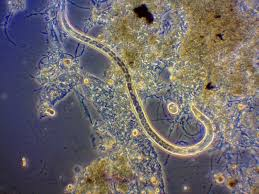
\includegraphics[scale=0.88]{Nematode} \end{center}\\
\begin{center} \textbf{Rotifer} \end{center} & \begin{center}\textbf{Nematode} \end{center}\\
\end{tabular}\\		
				
\begin{itemize}
\item The essence of the activated sludge system is to develop and and maintain a diverse population of microorganisms (activated sludge) that treats wastewater and which can be managed.
\item The activated sludge should be such that it \hl{not only effectively remove the BOD}, but also \hl{produces a floc that settles and compacts well} in the secondary clarifier thereby producing a secondary effluent with a low BOD content.
\item The floc produced has a porous structure and is essentially an aggregate of bacteria and extracelular material including organic polymers - polysaccharides and other substances secreted by the microorganisms, and remnants of dead microorganisms.  
\item Typically, the trophic organisms such as the protozoas and rotifers which feed on the bacteria and other particulates are generally present on the outer surface of the flocs.
\item A good quality activated sludge is brown in color with some froth and a slight musty odor.  
\item The settleability of the sludge is measured as SVI which is the volume of settled sludge in milliliters occupied by 1 gram of dry sludge solids after 30 minutes of settling in a 1,000 mL graduated cylinder or a settleometer.  
\item SVI of a good settling sludge is typically between 50 - 150 ml/g.\\ 
\item MCRT is the key factor which establishes the organism mix in the activated sludge.  
\item As MCRT increases, the size and complexity of the organisms increases.  
\item The types of organisms predominating in the mixed liquor give an indication as to the age of the sludge.
\begin{enumerate}[1.]  
\item At low MCRT of about less than 4 days the simpler protozoas - amoebae and flagellates dominate. 
\item With an increase in MCRT more complex organisms such as the free swimming ciliates and stalked ciliates appear. 
\item At even higher MCRT, metazoans such as the rotifers and nematodes may be found
\end{enumerate}
\end{itemize}
%Following is a chart showing the relative predominance of the trophic microorganisms with respect to the MCRT and its counterpart F:M.

%\begin{center}
%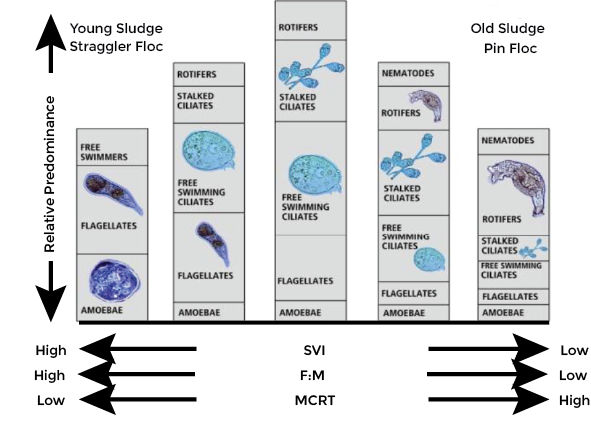
\includegraphics[scale=0.85]{ASRelativePredominance1}
%\end{center}


		\section{Activated sludge process control}\index{Activated sludge process control}	


\begin{itemize}
\item To ensure optimal treatment in the activated sludge process - maximum BOD removal with a well settling mixed liquor, controlling the inventory of solids (biomass) is a key process control parameter.\\
\item New solids (biomass) are produced in the activated sludge reactors due to the consumption of the BOD by the microorganisms.
\item The solids faction of the mixed liquor which separate (settle) in the secondary clarifier are
\begin{itemize}
\item Either returned to the influent end of the activated sludge reactor as Return Activated Sludge (RAS), or
\item removed from the system as Waste Activated Sludge (WAS). 
\end{itemize}
\item Thus, RAS and WAS pumping controls are used for maintaining the desired amount of solids in the system.
\end{itemize}

		\subsection{Controlling waste activated sludge (WAS) pumping rate}\index{Controlling waste activated sludge (WAS) pumping rate}	

For process stability and control the wasting should be continuous and not intermittent and any increase or decrease in wasting should be made gradually, i.e., 20 - 25 percent per day.  One of the following approaches is utilized to establish the WAS flow control 

		\subsubsection{Constant Mean Cell Residence Time (MCRT)}\index{Constant Mean Cell Residence Time (MCRT)}	


Typical MCRT for conventional AS process ranges from 5 to 15 days and 20 to 30 days for extended aeration and for a given plant, the desired MCRT is established based upon operational experience.  WAS flow control can be established to maintain the desired MCRT range for a given plant. 

		\subsubsection{Constant food:mass (F/M)}\index{Constant food:mass (F/M)}	

This parameter is based upon the ratio of food (influent BOD) fed to the microorganisms each day to the mass of microorganisms held under aeration. WAS flow control can be used for controlling the mass of microorganisms in the system to maintain the desired F/M ratio.

		\subsubsection{Constant Mixed Liquor Suspended Solids (MLSS)}\index{Constant Mixed Liquor Suspended Solids (MLSS)}	

A MLSS concentration which provides the best effluent and highest removal efficiencies is selected and WAS flow control is established to maintain the desired MLSS concentration level.  Wasting is increased when the MLSS concentration is higher and decreased or stopped when the MLSS concentration is lower than the desired level.

		\subsection{Controlling the return activated sludge (RAS) rate}\index{Controlling the Return activated sludge (RAS) rate}	

RAS flow rate affects the concentration and the sludge age.  
Return Activated Sludge Control...
To properly operate the activated sludge process,  For conventional activated sludge operations, the RAS flow is generally about 30 to 100\% of the incoming wastewater flow. Changes in the activated sludge quality will require different RAS flow rates due to settling characteristics of the sludge. The following approaches are used to control the RAS flow rate:

		\subsubsection{Constant RAS flow rate control - RAS pumping independent of influent flow}\index{Constant RAS Flow Rate Control - RAS pumping independent of influent flow}	

\begin{itemize}
\item Results in a continuously varying MLSS concentration that will be at a minimum during peak influent flows and a maximum during minimum influent flows. This occurs because the MLSS are flowing into the clarifier at a lower rate during peak flow when being removed at a constant rate. Similarly, at minimum influent flow rates, the MLSS are being returned to the aeration tank at a higher rate than are flowing into the clarifier
\item Maximum solids loading on the clarifier occurs at the initial start of peak flow periods.
\item The clarifier will have has a constantly changing depth of sludge blanket as the MLSS moves from the aeration tank to the clarifier and vice versa. 
\item This RAS control option is especially advantageous for smaller plants as it entails little effort/minimal automation for RAS pumping control.  
\item A disadvantage of using the constant flow approach is that the F/M is constantly changing. The range of F/M fluctuation due to the effect of short term variation in the MLSS (because of hydraulic loading) is generally small enough so that no significant problems arise due to using this approach.
\end{itemize}

		\subsubsection{Constant percentage RAS flow rate control}\index{Constant percentage RAS flow rate control}
\begin{itemize}
\item This approach requires a programmed method for maintaining a constant percentage of the aeration tank influent wastewater flow rate. The program may consist of an automatic flow measurement device, a programmed system, or frequent manual adjustments.
\item The variations in the MLSS concentration due to the diurnal flow profile are reduced and the F/M varies less.
\item The MLSS will remain in the clarifier for shorter time periods, which may reduce the possibility of denitrification in the clarifier.
\item Clarifier is subjected to maximum solids loading when the clarifier contains the maximum amount of sludge. This may result in solids washout with the effluent.\\
\end{itemize}

		\subsubsection{Establishing RAS flow rate based on a solids balance approach}\index{Establishing RAS flow rate based on a solids balance approach}
%Based upon a solids mass balance around the secondary clarifier, formula to calculate the Q\textsubscript{RAS} given Q, MLSS, and SS\textsubscript{RAS}
%
%$$Q\textsubscript{RAS} =(Q * MLSS - \dfrac{Q\textsubscript{WAS} * SS\textsubscript{RAS}}{(SS\textsubscript{RAS} - MLSS)}$$ 
The following equation can be used for controlling RAS flow rate to maintain a target MLSS concentration given the influent flow and the RAS solids content.\\
\vspace{0.3cm}
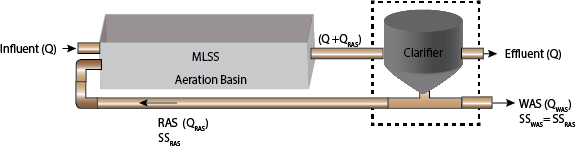
\includegraphics[scale=0.75]{RASQ}\\
Applying a mass balance approach to the secondary clarifier:\\
Mass of solids in = Mass of solids Out\\
$(Q + Q_{RAS})* MLSS = Q_{RAS} *SS_{RAS} + Q_{WAS} *SS_{RAS}$\\
Notes:
\begin{itemize}
\item The solids leaving with the effluent - $Q*SS_{EFF}$ is negligible\\
\item Also, $SS_{WAS}=SS_{RAS}$ \\
\end{itemize}
Rearranging:\\
%$ \implies Q*MLSS + Q_{RAS}*MLSS = Q_{RAS}* SS_{RAS} + Q_{RAS} *SS_{RAS}$\\
%$ \implies Q_{RAS}* SS_{RAS} - Q_{RAS}*MLSS =Q*MLSS - Q_{WAS} *SS_{RAS}$\\
%$ \implies Q_{RAS}*(SS_{RAS} - MLSS) = Q*MLSS - Q_{WAS} * SS_{RAS}$\\  
$ \implies Q_{RAS} = \Bigg(\dfrac{Q*MLSS - Q_{WAS} * SS_{RAS}}{SS_{RAS} - MLSS}\Bigg)$\\
As $Q_{WAS}*SS_{RAS}$ << $Q*MLSS$ and can be neglected\\
Rearranging:\\
$Q_{RAS} = \Bigg(\dfrac{Q*MLSS}{SS_{RAS} - MLSS}\Bigg)$ 
%OR $SS_{RAS} = \Bigg(\dfrac{(Q + Q_{RAS} )MLSS}{Q_{RAS}}\Bigg)$\\


\section{Process trouble shooting}\index{Process trouble shooting}

The most common activated sludge quality issues include:
\begin{enumerate}[1.]
\item Straggler floc:  This condition shows small, light, and fluffy floc particles with poor settling characteristics. It occurs due to young sludge or low MCRT/MLSS levels and may be related to an inadequate microorganism population or an excessive BOD load (high F:M) which causes a log growth situation. The cells become dispersed rather than flocculated, settleability is poor, and the effluent becomes turbid. In this condition oxygen is used up quickly due to the high metabolism rate, and sludge production is high. One tell-tale sign of this condition is the production of huge amounts of a billowing white foam.

\item Pin floc (Dispersed Growth):  Here flocs - pin floc is seen in the effluent. These are larger dimension spherical particles.  The sludge settles well in the settleability test but the supernatant is cloudy. This floc consist mostly of floc-forming bacteria without a filament backbone.  This condition occurs at starvation condition when all of the influent BOD has been used up (low F:M) and the old sludge age organisms are now in endogenous respiration.

\item Rising sludge: Under this condition, sludge settles well, compacts on the bottom of the clarifier, then starts to rise in clumps and patches to the surface.  Rising sludge is typically evidenced as brown in color.  Rising sludge occurs due to either denitrification or sludge septicity due to an excessive detention time in the clarifier.  

\item Bulking and foaming:  Typical bacteria present in activated sludge include spherical, rod shaped and filamentous.  The presence of filamentous bacteria in activated sludge provide the important structural element for the bacterial floc.  Bulking is indicated by SVI > 150 ml/g. However, certain condition cause an excessive growth of filaments which interferes with the settling (bulking) and cause foaming during aeration.   Identifying which filaments are dominating in the system through a microscopic evaluation will help the operator to understand the condition in the treatment system so that corrective changes can be made.
\end{enumerate}
\begin{center}

\includegraphics[scale=1.5]{Filaments}\\
Filaments proliferation
\end{center}


\begin{enumerate}[a.]

\item Bulking:  Activated sludge bulking is marked by poor compaction – high SVI\textsubscript{30} and poor solids-liquid separation evidenced by high effluent TSS.  To resolve bulking issue, it is important to find its cause and take remedial actions.  This is accomplished through a microscopic examination to identify the type of the filament to provide a clue on the cause.  Short term remedy to bulking includes Chlorinating – 2-3 mg/l per 1000 lbs MLVSS or use of polymers.

\item Foaming:  Activated sludge foaming is caused mostly by two filaments: Nocardia spp. and Microthrix parvicella (there are other non-filament causes of foaming - including excessive presence of surfactants. Both of these filaments have three causes in combination: (1) high grease and oil; (2) longer sludge age; and (3) low oxygen conditions or septicity.  Foaming if left uncontrolled could potentially pose a permit compliance issue if the foam spills into the effluent.  Additionally, Nocardia from the secondary sludge could cause digester foaming.
\end{enumerate}


\newpage
\thispagestyle{empty}
\begin{landscape}
\begin{table}[ht]
 % title of Table
\centering % used for centering table
\begin{tabular}{ | m {7 cm} | m {4 cm}| m {12 cm}| } 
 \hline
\begin{center}\textbf{Filament Type}  \end{center} & \begin{center} \textbf{Cause} \end{center} & \begin{center} \textbf{Remedy} \end{center}\\
 \hline
 S.natans, Type 1701 and H.hydrossis &  Low D.O. ( For the applied organic loading )&  Low aeration basin DO concentration for the applied F/M leads to filamentous bulking by several filaments.  Typically a minimum DO of 2 mg/l is required for F:M upto 0.5. The condition may also be remedies by raising the MLSS concentration (decreasing the F/M)\\ 
 \hline
 M.parvicella, Nocardia species, Type 0041, Type 0675, Type 1851 and Type 0803 &  Low Organic Loading Rate ( Low F:M )&  Increase the F:M by reducing the MLSS concentration. When reduction in the MLSS concentration may not be feasible due to impact on nitrification, other suitable methods such as the use of a selector may be considered\\
 \hline
 Thiothrix I and II, Beggiatoa species, N. limicola II, Type 021N, Type 0092, Type 0914, Type 0581, Type 0961 and Type 0411 &  Septic Wastes / Sulfides ( High organic acids ) &  Reduce septicity using pre-aeration and through use of chemicals which prevent septicity and reduce sulfides \\
 \hline
 Thiothrix I and II and Type 021N (N defeciency)
N. limicola III (P defeciency)&  Nutrient Deficiency ( N and / or P ) ( Industrial Wastes Only ) & \\
 \hline
Nocardia species, M.parvicella and Type 1863 & High Grease / Oil & \\
 \hline
 Fungi &  Low pH ( Below pH 6.0 ) / Oil  &  The aeration basin pH should be maintained in the range 6.5 to 8.5. Low pH, <6.5, may cause the growth of fungi and fungal bulking. The aeration basin pH can be adjusted using caustic, lime or magnesium hydroxide.\\
 \hline
\end{tabular}
\caption{Troubleshooting Activated sludge filaments}
\end{table}
\end{landscape}
\newpage


\section{Activated Sludge Process Modifications}\index{Activated Sludge Process Modifications}

\subsection{Conventional Activated Sludge Process}\index{Conventional Activated Sludge Process}

\noindent \textbf{Process Description}\\
\noindent The primary effluent (AS influent) - Q, along with the return activated sludge (RAS) - Q$_{RAS}$, are introduced at the head of the aeration tank.  The oxygen demand is the highest at this point and decreases uniformly as the wastewater travels from one end of the tank to the other.\\  


\begin{figure}[h!]
\begin{center}
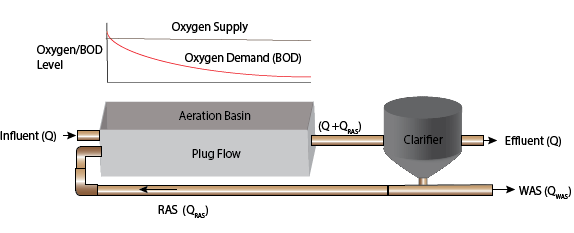
\includegraphics[height=5cm]{ConventionalActivatedSludge}
\caption{Conventional Activated Sludge Process}
\end{center}
\end{figure}

\noindent \textbf{Process advantages and applications}\\
The conventional activated sludge process is most suitable for low-strength, domestic wastes with minimal peak load considerations as this process is susceptible to failure from shock loads.  Shock Load is elevated strength (higher BOD and contaminant levels) in wastewater for brief period of time.\\

\textbf{Reasons for modifying the Conventional Activated Sludge Process}\\
Several factors contribute to the need for modifying the Conventional Activated Sludge Process:
\begin{itemize}
\item Unique characteristics of the influent flow which may include - high BOD loads, potential toxic loads, storm flows, loads with high carbonaceous BOD but low nitrogen
\item Space constraints
\item Energy and labor (O\&M) constraints
\item Constraints requiring low solids production
\end{itemize}

\subsection{Conventional Step Feed Process}\index{Conventional Step Feed Process}
\noindent \textbf{Process Description}\\
\noindent In this process modification, the primary effluent is fed to the aeration tank at several different locations within the tank.  The distribution of the influent along the length of the aeration reactor allows for distribution of the load (BOD) over the aeration tank and reduce oxygen sags in the aeration tank.  The return sludge is introduced separately from the primary effluent and in many cases is allowed a short re-aeration period  before mixing with primary effluent.\\

\begin{figure}[h!]
\begin{center}
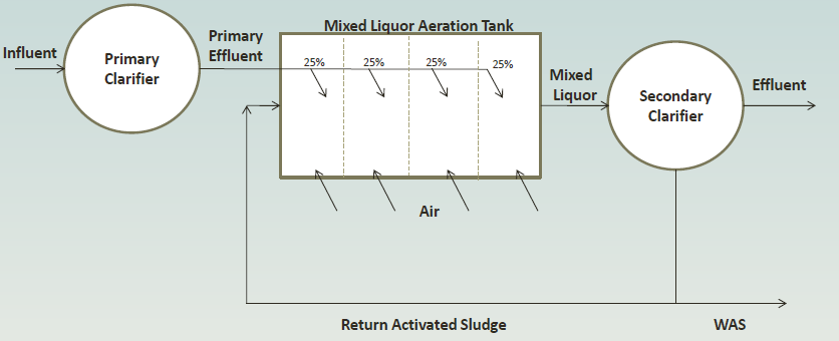
\includegraphics[height=4cm]{StepFeed}\\
\caption{Conventional Step Feed}
\end{center}
\end{figure}

\noindent \textbf{Process advantages and applications}
\begin{itemize}
\item Less aeration volume required to treat the same volume of wastewater compared to the conventional aeration.

\item Better control in handling shock loads

\item There is potential for:
\begin{itemize}
\item lower applied solids to the secondary clarifier
\item lower oxygen requirement
\end{itemize}
\item The step-feed process can be utilized on a variable basis using various modes (varying percent of the influent at the feed points) depending on the influent situation and the selection of the proper mode depends on the influent characteristics and the capabilities of the plant to handle the characteristics

\end{itemize}

\begin{figure}[bth!]
\begin{center}
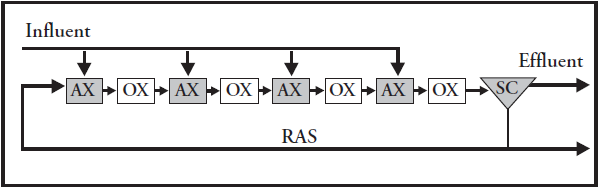
\includegraphics[height=3cm]{StepFeed1}\\
\caption{Step Feed Modification for Biological Nutrient Removal (BNR)}
\end{center}
\end{figure}



\subsection{Contact Stabilization}\index{Contact Stabilization}

\textbf{Process Description}
\begin{itemize}
\item This process modification requires two aeration tanks. 
\begin{enumerate}
\item Return Sludge Re-aeration tank:\\
\begin{itemize}
\item This tank is for separate re-aeration of the return activated sludge before it is mixed with the incoming wastewater
\item The residence time in the stabilization tank is typically 4 to 6 hours
\end{itemize}
\item Mixed Liquor Aeration tank (or Contact tank):\\
\begin{itemize}
\item This tank is for mixing of the primary effluent with the re-aerated return activated sludge
\item Here, the organisms quickly take in and store large amounts of food from the primary effluent.
\item The residence time in this tank is approximately 30 to 90 minutes
\end{itemize} 
\end{enumerate}
\end{itemize} 

\begin{figure}[h!]
\begin{center}
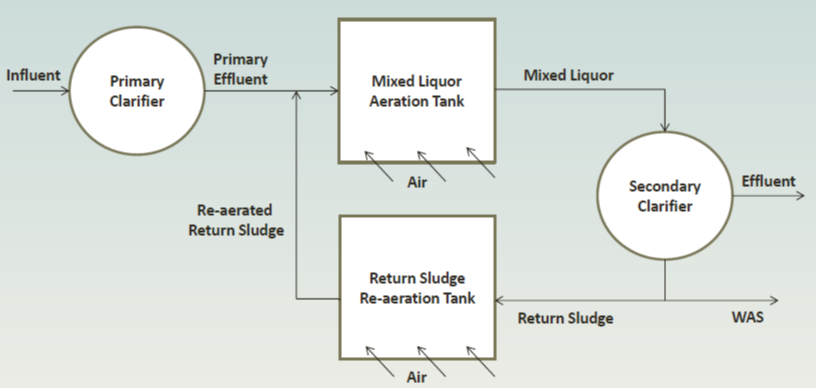
\includegraphics[height=6cm]{ContactStabilization}
\caption{Contact Stabilization}
\end{center}
\end{figure}


\noindent \textbf{Process advantages and applications}\\
Because the contact stabilization system has a reservoir of microbes in the re-aeration tank, it is better able to withstand solids washouts that accompany major storms and avoid microbial kill-offs related to short-term toxic dumps



\subsection{Pure Oxygen System}\index{Pure Oxygen System}

\noindent \textbf{Process Description}\\
\noindent Very similar to conventional activated sludge except that high purity oxygen is supplied to aeration tank (reactor) rather than air and this process treats more wastewater in a smaller space in a shorter period of time.  The Aeration tanks (reactors) are enclosed and sealed to prevent the oxygen from escaping from the tanks.  Pure oxygen from an oxygen generation system or is introduced in the headspace of the reactor.  Mechanical surface aerators agitate the mixed liquor (essentially splash the liquid in the headspace) to dissolve the oxygen into the mixed liquor.  High DO levels are maintained in the aeration tanks (4 mg/l to 15 mg/l).  Roughly 90\%-99\% gaseous O$_2$ goes in and 45-70\% gaseous O$_2$ is ventilated at the effluent end of the reactor.\\

\begin{figure}[h!]
\begin{center}
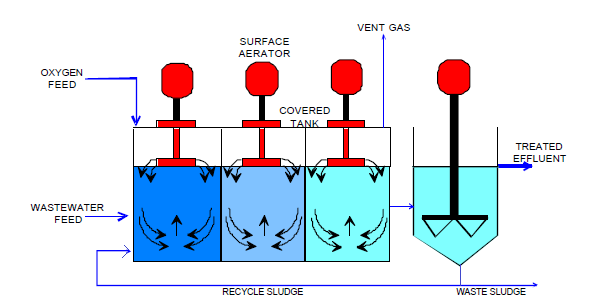
\includegraphics[height=6cm]{PureOx}
\caption{Pure Oxygen System}
\end{center}
\end{figure}

\noindent \textbf{Process advantages and applications}
\begin{itemize}
\item 
Pure oxygen systems are generally more stable and can treat large volumes of wastewater.  
\item It treats more wastewater in a smaller space in a shorter period of time
\end{itemize}



\subsection{Sequencing Batch Reactors}\index{Sequencing Batch Reactors}

\noindent \textbf{Process Description}\\
\noindent Rather than treating a continuous flow through a number of tanks, Sequencing Batch Reactors (SBRs) treat flows in “batches” through a single tank - "reactor" through sequencing stages.  It performs the same treatment steps as a conventional AS plant, but they do it in sequenced stages rather than in a continuous flow stream.  Most commonly preliminary treated wastewater is directly fed to the SBR.

\begin{figure}[h!]
\begin{center}
\tcbox{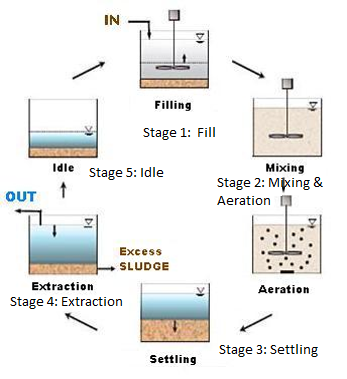
\includegraphics[height=10cm]{SBR}}
\caption{Sequencing Batch Reactor}
\end{center}
\end{figure}


Typically SBR is operated in five stages: 

\begin{enumerate}




\item Filling:  Influent raw wastewater enters the reactor 

\item Mixing \& Aeration:  This stage is where the BOD consumption and biomass production occurs.  Mixing and aeration may be alternated  to accomplish nitrification (during aeration) and denitrification (during mixing - without aeration - anoxic).

\item Settling - This is the clarification stage.  - to allow for the activated sludge floc to settle.

\item Extraction - in this stage the supernatant treated wastewater is removed (for disposal) and part of the settled sludge is wasted.

\item Idle - This stage is essentially to prepare the reactor and the biomass to receive the raw wastewater - Filling stage.  In this stage some aeration/mixing may be provided.  The biomass in the reactor enters the endogenous phase as the food is absent.  The biomass metabolizes the stored food and the organisms feed on one another.
\end{enumerate}


\noindent \textbf{Process advantages and applications}
\begin{itemize}
\item SBRs are ideal for small facilities as the process can be easily automated

\item SBRs are very stable due to the high sludge ages maintained and the fact that all treatment takes place in a single tank

\item SBR construction is less costly due to the elimination of secondary clarifiers and sometimes digestion facilities (fewer structures in general)
\end{itemize}


\subsection{Extended Aeration}\index{Extended Aeration}

\begin{figure}[h!]
\begin{center}
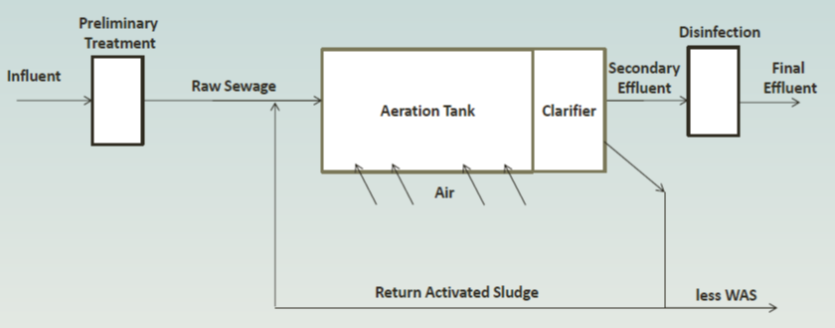
\includegraphics[height=5.5cm]{ExtendedAeration}
\caption{Extended Aeration}
\end{center}
\end{figure}

\noindent \textbf{Process Description}\\
\noindent This process typically directs raw sewage flow (without grit/screenings) into the aeration tank where it undergoes treatment for an extended period (usually 8 hours or more – 15 hours typical) followed by clarification.  Mixed liquor concentrations are usually maintained at high concentrations.  Typical F:M ratios are about 0.05 to 0.15 and MCRT of about 30 days.\\

\noindent \textbf{Process applications and advantages}
\begin{itemize}
\item This process modification is appropriate for small facilities that have light solids loadings – plants typically treating less than 1 MGD – as the aeration tank volume requirement is larger
\item In addition to consuming all the incoming food, the microbes consume all food stored within cells - endogenous respiration, and other dead microbes in the system
\item Extended aeration does not produce as much waste sludge as other process modifications
\item The oxidation ditch is a variation of the extended aeration process.  In the oxidation ditch, the aeration basin is ring or oval shaped.  Aeration rotors or brushes cause the wastewater to flow around the ring and also aerate the wastewater.
\end{itemize}

\begin{figure}[h!]
\begin{center}
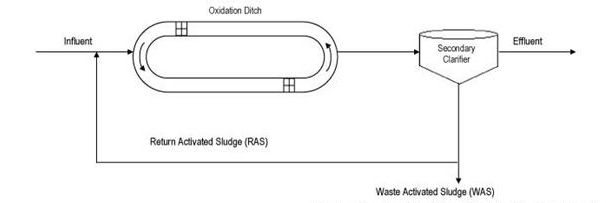
\includegraphics[height=3cm]{OxidationDitch}
\caption{Extended Aeration - Oxidation Ditch}
\end{center}
\end{figure}



\subsection{Krauss Process}\index{Krauss Process}

\noindent \textbf {Process Description}\\
\noindent The process involves use of two aeration tanks.  One aeration tank (Aeration Tank B in the graphic), is for blending return activated sludge (RAS) with anaerobic digester supernatant or sludge and aerating the solution.  The other tank receives primary effluent (Aeration Tank A), return activated sludge, and the aerated mixture of return sludge and digester supernatant/sludge.  Air (oxygen) is added to both aeration tanks.\\

\begin{figure}[h!]
\begin{center}
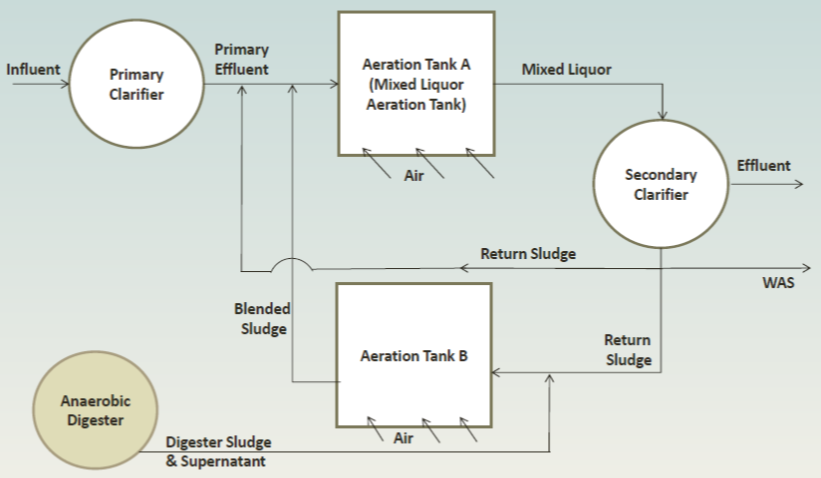
\includegraphics[height=5.5cm]{Kraus}
\caption{Krauss Process}
\end{center}
\end{figure}

\noindent \textbf{Process advantages and applications}\\
This process modification is widely used when wastewater contains a high ratio of carbonaceous to nitrogenous material in the wastewater (nitrogen deficient).  This typically occurs when there is significant contribution of wastewater from canneries or dairies.  When the little nitrogen present in the influent wastewater is consumed, further consumption of carbonaceous material ceases.  The digester supernatant or sludge being typically rich in nitrogenous material provides the required nitrogen for the nitrogen deficient process stream.


\section{Activated sludge math problems}\index{Activated sludge math problems}
\subsection{MCRT (Mean Cell Residence Time}\index{MCRT (Mean Cell Residence Time}


\vspace{0.2cm}
The MCRT is calculated as:\\  
\vspace{0.2cm}
$MCRT(days) = $\\
$\dfrac{Total \enspace MLSS \enspace lbs \enspace in \enspace the \enspace aeration \enspace system \enspace (aeration \enspace tank \enspace + \enspace clarifier)}{Total \enspace amount \enspace in \enspace lbs/day \enspace of \enspace suspended \enspace solids \enspace leaving  \enspace the \enspace system \enspace(Effluent\enspace SS+ WAS \enspace solids)}$\\
\vspace{0.4cm} 
$MCRT (days) = \dfrac{MLSS \enspace in \enspace aeration \enspace tank \enspace (lbs)+MLSS \enspace in \enspace clarifier \enspace (lbs)}{Effluent \enspace suspended \enspace solids \enspace (lbs/day)+\enspace WAS \enspace SS \enspace (lbs/day)}$\\
\vspace{0.3cm}
\textbf{Key Points for Solving MCRT Problems}\\
\begin{enumerate}
\item \textbf{MLSS quantification}:\\ 
\begin{itemize}
\item Pounds formula is used to calculate lbs MLSS using: i) aeration tank and the clarifier volumes, and ii) the given MLSS concentration.  
\item The MLSS concentrations for the aeration tank and the clarifier are the same.  So the given MLSS concentration applies to both - the aeration tank and the clarifier
\item Make sure it is the MLSS concentration that you are using not the MLVSS concentration.  
\item If MLSS concentration is not given but instead MLVSS concentration is given, you will need to find the MLSS concentration by dividing the MLVSS conc. by the mixed liquor volatile solids, as MLVSS(conc.) = MLSS * \% volatile solids
\end{itemize}

\item \textbf{Suspended solids quantification}:\\ 
\begin{enumerate}
\item \textbf{Effluent suspended solids}
\begin{itemize}
\item Effluent suspended solids can be quantified using the pounds formula - using the effluent flow (in MGD) and the effluent suspended solids concentration.
\end{itemize}
\item \textbf{WAS suspended solids}
\begin{itemize}
\item Use pounds formula given the WAS flow (make sure it is in MG) and the WAS SS concentration
\item Note that the WAS and RAS streams have the same SS concentration.  If WAS SS concentration is not specified, use the RAS SS concentration
\end{itemize}
\end{enumerate}
\end{enumerate} 

\hl{Example Problems:}\\
\begin{enumerate}
\item In an conventional activated sludge plant  the aeration tank contains 6000 lbs of MLSS and the final clarifier contains 2300 lbs of MLSS. 1450 lbs of solids are wasted each day and 90 lbs/day of solids leave in the final effluent. Calculate the MCRT for this plant.\\
Solution:\\
\vspace{0.2cm} 
$MCRT (days) =  \dfrac{MLSS \enspace in \enspace aeration \enspace tank \enspace (lbs)+MLSS \enspace in \enspace clarifier \enspace (lbs)}{SS \enspace effluent \enspace (lbs/day)+SS \enspace WAS \enspace (lbs/day)}$\\
\vspace{0.2cm} 
$MCRT (days) =  \dfrac{6000lbs \enspace + \enspace 2300 lbs}{90lbs/day\enspace + \enspace 1450 lbs/day}=5.4=\boxed{5days}$\\
\vspace{0.3cm} 
\item A activated sludge plant treats an average influent flow of 4 MGD.  The plant has two  aeration tanks – 0.45 MG volume each and two final clarifiers – 0.2 MG volume each, and a mixed liquor suspended solids concentration averages  1800 mg/l.   The effluent suspended solids concentration averages 18 mg/L. The WAS flow is 100,000 gallons per day has a SS concentration of 6100 mg/L. Calculate the MCRT\\
Solution:\\
$MCRT (days) =  \dfrac{MLSS \enspace in \enspace aeration \enspace tank \enspace (lbs)+MLSS \enspace in \enspace clarifier \enspace (lbs)}{SS \enspace effluent \enspace (lbs/day)+SS \enspace WAS \enspace (lbs/day)}$\\
\vspace{0.3cm} 
$MLSS \enspace in \enspace aeration \enspace tank \enspace (lbs)=2*0.45*1800*8.34=13511lbs$\\
\vspace{0.3cm} 
$MLSS \enspace in \enspace clarifier \enspace (lbs)=2*0.2*1800*8.34=6005lbs$\\
\vspace{0.3cm} 
$SS \enspace effluent \enspace (lbs/day)=4MGD *18mg/l*8.34=600lbs/day$\\
\vspace{0.3cm} 
$SS \enspace WAS \enspace (lbs/day)=\dfrac{100000}{1000000}MGD *4800mg/l*8.34=4003lbs/day$\\
\vspace{0.3cm} 
Plugging in the values calculated above: $MCRT (days) =  \dfrac{13511+6005}{600+4003}=4.2=\boxed{4days}$\\
\end{enumerate}

\subsection{F:M (Food to Microorganism Ratio}\index{F:M (Food to Microorganism Ratio}
\begin{itemize}
\item This parameter ratios the food – the mass of primary effluent BOD entering the aeration basin to the mass of the microorganisms - \textbf{MLVSS}, in the aeration basin.
\item \textbf{Only the mass of the microorganisms (MLVSS) in the aeration basin is used – the mass of microorganisms in the secondary clarifier is not considered}
\item Common ranges for F/M for a conventional activated sludge plant are from 0.15 to 0.5. 
\item The optimum F/M varies from plant to plant and can be determined by trial and error.
\item The F:M may be used to determine the concentration of mixed liquor suspended solids to be maintained in the aeration tank.
\item Generally, low F/M ratios should be carried during the colder months as the microorganism activity (metabolism) is lower.
\item F:M and MCRT are inversely related: that is a long MCRT means a low F:M and a short MCRT means a high F:M
\end{itemize}
F:M=$\dfrac{amount \enspace of \enspace food \enspace coming \enspace in}{amount \enspace of \enspace microorganisms \enspace present}$\\
\vspace{0.3cm}
\hspace{0.7cm}$=\dfrac{(lbs/day) \enspace primary \enspace effluent  \enspace BOD \enspace entering \enspace the  \enspace aeration \enspace tank}{(lbs) \enspace MLVSS \enspace in \enspace the  \enspace aeration \enspace tank}$\\
\vspace{0.3cm}
\textbf{Key Points for Solving F:M Problem}\\
\begin{enumerate}
\item \textbf{Quantifying F:}
\begin{itemize}
\item use the pounds formula to calculate the lbs/day of BOD in the primary effluent.\\
lbs/day BOD = Primary eff. flow (MGD)* Primary eff. BOD concentration (mg/l) * 8.34\\
\end{itemize}
\item \textbf{Quantifying M:}
\begin{itemize}
\item The concentration of the microorganisms is assumed to be the same as the MLVSS concentration
\item \textbf{Only the mass of the microorganisms (MLVSS) in the aeration basin is used – the mass of microorganisms in the secondary clarifier is not considered} 
\item lbs MLVSS may be calculated using pounds formula using the volume of the aeration tank (in MG) and the MLVSS concentration
\item If the MLVSS concentration is not given, it can be calculated from the MLSS and MLSS \% volatile matter (solids) concentration\\
MLVSS = MLSS * \% MLSS volatile solids
\end{itemize}


\hl{Example Problem:}\\
\begin{enumerate}[i.]
\item A conventional activated sludge plant receives an average flow of 5.5 MGD. The influent BOD to the plant averages 230mg/l and the primary effluent BOD average 160 mg/l. The 1 MG aeration tank has an MLSS concentration of 2800 mg/L and the MLVSS volatile solids content is 75\%. Calculated the F:M ratio for this plant.
\vspace{0.3cm}
Solution:\\
\vspace{0.3cm}
F=5.5*160*8.34=7339lbs/day BOD\\
M=1*2800*0.75*8.34=17514lbs MLVSS\\
F:M=$\dfrac{7339}{17514}=\boxed{0.41}$\\

Note:  The 160 mg/l BOD concentration of the primary effluent was used for the F calculation and not 230mg/l - which is the BOD concentration of the flow coming into the plant\\
\end{enumerate}

\subsection{Sludge Volume Index (SVI)}\index{Sludge Volume Index (SVI)}

\begin{itemize}
\item SVI measures the settleability and compactibility of the secondary sludge
\item It is calculated using results from the 30-minute settleability test and the MLSS concentration
\item SVI is expressed in ml/g and it is essentially the volume (ml) of 1 gram of the MLSS after 30 minutes of settling
\item it provides a more accurate picture of the sludge settling characteristics than settleability or MLSS alone
\item 50 to 120 ml/gm SVI value is considered
optimal. Higher SVI values indicate sludge that is slow to settle and not compacting well. When SVI
values are approaching 200 ml/gm, activated sludge process is considered to be "bulking".
\end{itemize}
\end{enumerate}
SVI (ml/g)= $\dfrac{Settled \enspace sludge \enspace volume \enspace in \enspace ml/l \enspace after \enspace 30 \enspace min}{MLSS \enspace mg/l}*1000 \dfrac{mg}{g}$\\
\vspace{0.3cm}
\textbf{Key Points for Solving SVI Problems}\\
\begin{itemize}
\item For the settling test MLSS is typically settled in a 1 liter settleometer.  The volume of the settled solids is therefore read as ml/L.  So if for any reason a larger or smaller volume of the mixed liquor sample is taken, the settle solids value should commensurate with the volume of the MLSS sample.  For example, if a 2 liter settleometer is used and if the solids settle to 400 ml in that settleometer, the ml/L will be 400ml/2L or 200ml/L
\item For some problems, the settled solids volume is provided as a percentage (\%).  So if a 1-liter settlometer is used and the settled solids volume is reported as 25\%, it implies a settled sludge volume of 250ml/L
\end{itemize} 
\hl{Example Problem:}\\
\begin{enumerate}[i.]
\item In an aeration tank, the MLSS is 2500 mg/l and recorded 30-minute settling test indicates 230 ml/L.  What is the sludge volume index?\\
\vspace{0.3cm}
Solution:\\
SVI=$\dfrac{230ml/l}{2500mg/l}*1000\dfrac{mg}{g}=\boxed{92ml/g}$

\end{enumerate}





